\documentclass{notes2}
\usepackage{physics}
\usepackage{amsmath}
\usepackage{amssymb}
\usepackage[backend=bibtex, style=authoryear]{biblatex}
\addbibresource{Optimal_Pulse_Control.bib}
\title{GRAPE for Ion Trap System}
\author{Kun-Long Wu}
\newcommand{\closef}{\mathbf{F}}
\newcommand{\openf}{\mathcal{F}}
\newcommand{\dvbar}[1]{\overline{#1}}
\begin{document}

\maketitle
\tableofcontents

\newpage
\section{GRAPE}
\begin{align*}
    U_k = \mathcal{T}\exp\left\{(-i\tau)\int_{t_k}^{t_k+\tau}\dd s\mathcal{H}(s)\right\} \approx \exp\{-i\tau H(t_k)\} + O(\tau^2 \norm{H}^2) \\
\end{align*}
We require $\kappa_1 = \tau \norm{H}\ll 1$.
\section{Noise: Fluctuation and Decoherence}
Additional to the original parametrized hamiltonian, we also consider the uncertainty of the system. The hamiltonian is than consider as a function of random variable $\xi$:
\begin{equation}
    H(t; \vb* \xi, \vb* \chi) = H_0(t) + \sum_m \xi_m(t) \cdot H_{\xi_m}+ \sum_{i} c_i(t) [H_i + \chi_i(t) H_{\chi_i}]
    \label{eq:total_hamiltonian}
\end{equation}
where $\xi$ and $\chi$ are random variables that describe the fluctuation of the system with mean value zero.

Two limits of time correlation of the fluctuation are considered. The first one is the limit of infinitely long time correlation, i.e., $\xi$ is a random variable that is constant during the whole gate operation. The second one is the limit of infinitely short time correlation, i.e., $\xi$ is a random variable that is independent at different time.
The correlation function for each are 
\begin{align}
    \text{long time correlation (fluctuation): } &\expval{\xi_j(t)\xi_j(t')} = \sigma^2 \\
    \text{short time correlation (decoherence): } &\expval{\xi_j(t)\xi_j(t')} = \sigma^2 \delta(t - t')
\end{align}
Long time correlation is considered as the fluctuation of the system, while short time correlation is considered as the markovian noise of the system, which can be described by the Lindblad master equation.
Thus the evolution of the system can be described by the following equation:
\begin{equation}
    \dot \rho = -i[H(t; \vb* \xi, \vb* \chi), \rho] + \sum_j  (L_j \rho L_j^\dagger - \frac{1}{2} L_j^\dagger L_j \rho - \frac{1}{2} \rho L_j^\dagger L_j)
\end{equation}
Lindblad gives from the short time correlation limit, and the $\xi,\chi$ reduced to time-independent random variable that only has long time correlation.

\section{Gate Fidelity and Cost Function}
Let $F$ be the close gate fidelity that does not include the effect of fluctuation and noise, and $\mathcal{F}$ be the open gate fidelity that faithfully describe the system under fluctuation and noise. $\mathcal{J}$ be the real function that we actually minimize.
\begin{align*}
    \closef &= \frac{1}{N} \sum_{p,q}\bra{p,q}\hat U^\dagger U(0, T; \vb c)\ketbra{p_0,q} U(0, T; \vb c)^\dagger \hat U \ket{p,q}\\
    \openf &= \frac{1}{N} \sum_{p,q}\expval{\bra{p,q}\hat U^\dagger {\mathcal{E}_\xi}\left(\ketbra{p_0,q};\vb c\right)\hat U \ket{p,q}}\\
    \mathcal{J} &= 1 - \openf + \lambda L_1
\end{align*}
the set of $q$ spans the logical subspace. For two qubits gate, the logical subspace is spanned by $\{\ket{0}, \ket{1}, \ket{+}, \ket{-}, \ket{+i}, \ket{-i}\}^{\otimes 2}$. Thus $N = 36$.



\subsection{Gradient with Fluctuation}
Consider the hamiltonian with fluctuation, we can write the evolution of the system as:
\begin{equation}
    U = \exp\{-i\tau H + H_f\}
\end{equation}
Focusing on $\mathcal{E}_\xi$, we can write it as the following form:
\begin{align}
    \mathcal{E}_\xi(\rho_0) &= (U_N + \delta U_N) \cdots (U_1 + \delta U_1) \rho_0 (U_1^\dagger + \delta U_1^\dagger) \cdots (U_N^\dagger + \delta U_N^\dagger)\\
    \begin{split}
    = U_N \cdots U_1 \rho_0 U_{-1} \cdots U_{-N} + \sum_{j=-N, j\neq 0}^N U_N \cdots \delta U_j \cdots U_1 \rho_0 U_{-1} \cdots U_{-N} \\
    + \sum_{i,j=-N, i,j\neq 0}^N U_N \cdots \delta U_i \cdots \delta U_j \cdots U_1 \rho_0 U_{-1} \cdots U_{-N} + \cdots
    \end{split}\label{eq:fluc_expansion_E}
\end{align}

where $\delta U_j = -i\tau\vb*\xi\cdot \vb H_{\xi}U_j$ is the first order perturbation of the propagator $U_j$ due to the fluctuation.
We notice that the expectation of the first order term is zero, thus the leading order of the fluctuation effect is the second order term, i.e., $\expval{\mathcal{E}_\xi - \mathcal{E}} \approx \sum_{i,j=-N, i,j\neq 0}^N \expval{U_N \cdots \delta U_i \cdots \delta U_j \cdots U_1 \rho_0 U_{-1} \cdots U_{-N}}$. This can be evaluated by the correlation function of the noise. For fluctuation with long time correlation, we have $\expval{\xi_j(t)\xi_j(t')} = \sigma^2$, thus it becomes a function of standard deviation $\sigma$ of the fluctuation.

Define $W$ as the propagator without fluctuation terms.
\begin{equation}
    W_j = \exp\left\{-i\tau \left(H_0(t_j) + \sum_{i} c_i(t_j) H_i \right)\right\} + O(\tau \abs{H})
\end{equation}
Define $V$ as  the first order perturbation of the propagator $U_j$ due to the fluctuation
\begin{equation}
V_j = -i\tau(\sum_i\sigma_{\xi_i} H_{\xi_i}+ \sum_i\sigma_{\chi_i} c_i(j) H_{\chi_i}) W_j
\end{equation} 
we can get the following expansion of the open gate fidelity to first non-vanishing order of the fluctuation, i.e., the second order of $V$:
\begin{equation}
    \openf \approx \closef + \sum_{i,j=-N}^N \bra{\psi} W_{N} \cdots V_{i} \cdots W_1 W_0 W_{-1} \cdots V_j \cdots W_{-N} \ket{\psi}\qquad (i>j,\, i,j\neq 0)
    \label{eq:fluc_expansion_a}
\end{equation}
where $W_0 = \ketbra{\psi_0}$, $W_{-1} = W_{1}^\dagger$. Notice that the perturbation expansion is valid (converge) only when $\kappa_2 = \sigma\norm{H_{\text{fluc}}} T < 1$. A good approximation for the first order approximation further requires $(\sigma\norm{H_{\text{fluc}}} T)^2 \ll 1$.

To calculate the derivative of the open gate fidelity, we need first define following six states group, for $k = 1, 2,\ldots, N$:
\begin{itemize}
    \item $\ket{F_k} = W_k\cdots W_1\ket{\psi_0}$ for the forward propagation of the initial state with no fluctuation
    \item $\ket{SF_k} = \sum_{i=1}^k W_k\cdots W_{i+1}V_i W_{i-1} \cdots W_1\ket{\psi_0}$ for the forward propagation with a single fluctuation. $\ket{SF_k} = 0$ if $k = 0, 1$
    \item $\ket{DF_k} = \sum_{i,j}W_k\cdots V_i \cdots V_j \cdots W_1\ket{\psi_0}$ for the forward propagation with double fluctuation
    \item $\bra{B_k} = \bra{\psi_T} W_N \cdots W_{k+1}$ for the backward propagation of the target state with no fluctuation
    \item $\bra{SB_k} = \sum_{j}\bra{\psi_T} W_N \cdots V_j \cdots W_{k+1}$ for the backward propagation with a single fluctuation
    \item $\bra{DB_k} = \sum_{i,j}\bra{\psi_T} W_N \cdots V_i \cdots V_j \cdots W_{k+1}$ for the backward propagation with double fluctuation
\end{itemize}
Then open fidelity can be decomposed by thinking of putting two indistinguishable $V$ to 4 different positions
\begin{itemize}
    \item $\ket{SF_k} = W_k\ket{SF_{k-1}} + V_k \ket{F_{k-1}}$
    \item $\ket{DF_k} = W_k\ket{DF_{k-1}} + V_k \ket{SF_{k-1}}$
\end{itemize}
\begin{figure}[h]
    \centering

    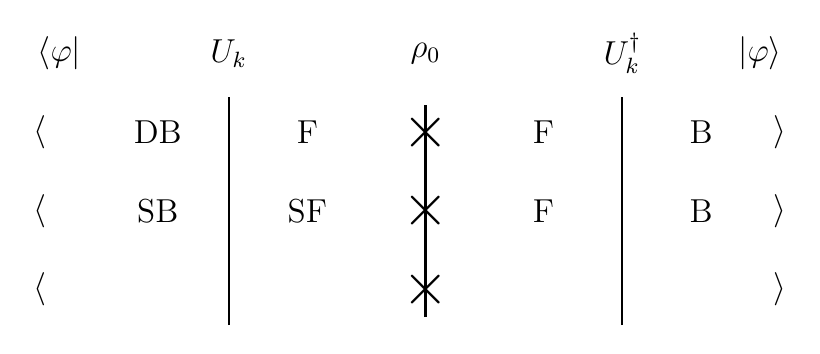
\begin{tikzpicture}[
    font=\large,
    every node/.style={inner sep=2pt},
]
% ---- column x-coordinates ----
\def\xbra{0}      % <phi|  and the three < bras
\def\xlab{1.5}    % DB / SB labels
\def\bL{2.4}      % left vertical bar of inner bracket
\def\xUk{3.4}     % U_k entries (F / SF)
\def\xrho{4.9}    % rho_0 spine with the three crosses
\def\xUkd{6.4}    % U_k^dagger entries (F / Fbar)
\def\bR{7.4}      % right vertical bar of inner bracket
\def\xB{8.4}      % |phi> entries (B / B)
\def\xket{9.4}    % the three > kets
 
% ---- row y-coordinates ----
\def\yh{3}        % header row
\def\yA{2}        % row 1
\def\yB{1}        % row 2
\def\yC{0}        % row 3
 
% ---- header labels ----
\node at (\xbra+0.25,\yh) {$\langle\varphi|$};
\node at (\bL  ,\yh) {$U_k$};
\node at (\xrho,\yh) {$\rho_0$};
\node at (\bR  ,\yh) {$U_k^{\dagger}$};
\node at (\xB+0.75,\yh) {$|\varphi\rangle$};
 
% ---- left bras ----
\node at (\xbra,\yA) {$\langle$};
\node at (\xbra,\yB) {$\langle$};
\node at (\xbra,\yC) {$\langle$};
 
% ---- DB / SB labels ----
\node at (\xlab,\yA) {DB};
\node at (\xlab,\yB) {SB};
 
% ---- left vertical bar ----
\draw[thick] (\bL,\yC-0.45) -- (\bL,\yA+0.45);
 
% ---- U_k column ----
\node at (\xUk,\yA) {F};
\node at (\xUk,\yB) {SF};
 
% ---- rho_0 spine with three crosses ----
\draw[thick] (\xrho,\yC-0.35) -- (\xrho,\yA+0.35);
\node[scale=1.8] at (\xrho,\yA) {$\times$};
\node[scale=1.8] at (\xrho,\yB) {$\times$};
\node[scale=1.8] at (\xrho,\yC) {$\times$};
 
% ---- U_k^dagger column ----
\node at (\xUkd,\yA) {F};
\node at (\xUkd,\yB) {F};   % second entry: change to {F} if it is just a plain F
 
% ---- right vertical bar ----
\draw[thick] (\bR,\yC-0.45) -- (\bR,\yA+0.45);
 
% ---- |phi> column ----
\node at (\xB,\yA) {B};
\node at (\xB,\yB) {B};
 
% ---- right kets ----
\node at (\xket,\yA) {$\rangle$};
\node at (\xket,\yB) {$\rangle$};
\node at (\xket,\yC) {$\rangle$};
 
    \end{tikzpicture}
\caption{The fluctuation summation can be decomposed as follows: the propagation chain is partitioned by $U_k$, $\rho_0$, and $U_k^\dagger$, which defines four possible insertion regions for each fluctuation operator. The two indistinguishable $V$ operators may be placed either in the same region or in different regions. In each region, the contribution can be double fluctuation ($DF$ or $DB$), single fluctuation ($SF$ or $SB$), or no fluctuation ($F$ or $B$). It is also worth to note that at second order, each chain contains exactly two fluctuation operators. }
\end{figure} we have total of 11 different terms.


\begin{align*}
    F = B^\dagger FF^\dagger B\\
    \mathcal{F} = F + &DB^\dagger\, F\, F^\dagger\, B + h.c.\\
    + &SB^\dagger\, SF\, F^\dagger\, B + h.c.\\
    + &SB^\dagger\, F\, SF^\dagger\, B + h.c.\\
    + &SB^\dagger\, F\, F^\dagger\, SB \\
    + &B^\dagger\, DF\, F^\dagger\, B + h.c.\\
    + &B^\dagger\, SF\, SF^\dagger\, B
\end{align*}
\begin{align*}
    \mathcal{\overline{F}} = \dvbar{F}{c} = 2\mathbf{Re}\{B^\dagger \dvbar{F}F^\dagger B + DB^\dagger \dvbar{F}F^\dagger B + B\dvbar{F}F^\dagger DB + \cdots\}
\end{align*}
Introduce the notation
\begin{equation}
    \dvbar{F_k} = \pdv{\ket{F_k}}{\vb c(k)}
\end{equation}
Now the derivative can be calculated by $\dvbar{F}$, $\dvbar{SF}$, $\dvbar{DF}$.

\begin{align*}
    \dvbar{F_k} &= \pdv{W_k}{\vb c(k)} W_{k-1} \cdots W_1 \ket{\psi_0} = -i\tau H_c \ket{F_k} = \dvbar{W_k}\ket{F_{k-1}}\\
    \dvbar{SF_k} &= \sum_{i=1}^{k-1} \pdv{W_k}{\vb c(k)} W_{k-1} \cdots W_{i+1}V_i W_{i-1} \cdots W_1\ket{\psi_0} + \pdv{V_k}{\vb c(k)}W_{k-1} \cdots W_1\ket{\psi_0} \\
    &= \dvbar{W_k}\ket{SF_{k-1}} + \dvbar{V_k}\ket{F_{k-1}} \\
    \dvbar{DF_k} &= \sum_{i,j}^{k-1} \pdv{W_k}{\vb c(k)} W_k \cdots V_i \cdots V_j \cdots W_1\ket{\psi_0} + \sum_{i}\pdv{V_k}{\vb c(k)}W_{k-1}\cdots V_{i}\cdots W_1\ket{\psi_0} \\
    &= \dvbar{W_k}\ket{DF_{k-1}} + \dvbar{V_k}\ket{SF_{k-1}}
\end{align*}

The derivative of the propagator $W$ and $V$ can be calculated by the Frechet derivative of the matrix exponential. With the condition $\kappa_1\ll 1$, we can get the expansion of Dyson and remain the first order term. 
\begin{align}
    \pdv{W_k}{c_i(j)}
    &=
    -i\tau H_i W_k
    + O\!\left((\tau\norm{H})^2\right),
    \\
    \pdv{V_k}{c_i(k)}
    &=
    -i\tau \sigma_{\chi_i} H_{\chi_i}W_k
    + (-i\tau)^2
    \left(
        \sigma_{\xi}H_{\xi}
        + \sigma_{\chi}c(j)H_{\chi}
    \right)
    H_i W_k + O\!\left((\tau\norm{H})^3\right) ,
    \notag\\
    &=
    -i\tau \sigma_{\chi_i}H_{\chi_i}W_k
    + O\!\left((\tau\norm{H})^2\right) .
\end{align}

\[\sigma_k=\sqrt{\sum_j \|H_{\mathrm{static},j}\|_2^2+\sum_a\left(
c_{k,a}\|H_{\mathrm{control\_fluc},a}\|_2
\right)^2}
\]


\[
\sigma_{\mathrm{rms}}
=
\sqrt{
\frac{1}{N}
\sum_k \sigma_k^2
}
\]
The leading order of the fluctuation effect is $(\sigma_{\mathrm{rms}}T)^2$, define $\kappa_2 = \sigma_{\mathrm{rms}}T$, we require $\kappa_2^2 \ll 1$ for the first order approximation to be valid.


\subsection{Decoherence Term}
For the short time correlation part, the noise is Markovian and is described
by the Lindblad superoperator
\begin{equation}
    \dot{\rho}(t)
    =
    -i[H(t),\rho(t)]
    +
    \mathcal{L}[\rho(t)] .
    \label{eq:lindblad_master_for_decoherence}
\end{equation}
Let $U(t,0)$ be the Hamiltonian propagator,
\begin{equation}
    i\dv{}{t}U(t,0) = H(t)U(t,0),
    \qquad
    U(0,0)=I.
\end{equation}
The closed-system trajectory is
\begin{equation}
    \rho_0(t)
    =
    U(t,0)\rho(0)U^\dagger(t,0).
\end{equation}
To isolate the decoherence contribution, move to the Hamiltonian interaction
picture:
\begin{equation}
    \rho(t)
    =
    U(t,0)\widetilde{\rho}(t)U^\dagger(t,0),
    \qquad
    \widetilde{\rho}(t)
    =
    U^\dagger(t,0)\rho(t)U(t,0).
\end{equation}
Then the Hamiltonian part is removed and the remaining evolution is
\begin{equation}
    \partial_t\widetilde{\rho}(t)
    =
    \widetilde{\mathcal{L}}(t)[\widetilde{\rho}(t)],
\end{equation}
where the interaction-picture Lindblad superoperator is
\begin{equation}
    \widetilde{\mathcal{L}}(t)[\widetilde{\rho}]
    =
    U^\dagger(t,0)
    \mathcal{L}\!\left[
        U(t,0)\widetilde{\rho}U^\dagger(t,0)
    \right]
    U(t,0).
\end{equation}

The integral equation is
\begin{equation}
    \widetilde{\rho}(T)
    =
    \widetilde{\rho}(0)
    +
    \int_0^T
    \widetilde{\mathcal{L}}(s_1)[\widetilde{\rho}(s_1)]\dd s_1 .
\end{equation}
Iterating this equation gives a Dyson expansion in the decoherence strength:
\begin{align}
    \widetilde{\rho}(T)
    =
    \widetilde{\rho}(0)
    &+
    \int_0^T
    \widetilde{\mathcal{L}}(s_1)[\widetilde{\rho}(0)]\dd s_1
    \notag\\
    &+
    \int_0^T\dd s_1
    \int_0^{s_1}\dd s_2\,
    \widetilde{\mathcal{L}}(s_1)
    \widetilde{\mathcal{L}}(s_2)
    [\widetilde{\rho}(0)]
    + \cdots .
    \label{eq:lindblad_dyson_expansion}
\end{align}
Keeping only the first order decoherence correction,
\begin{equation}
    \widetilde{\rho}(T)
    \approx
    \rho(0)
    +
    \int_0^T
    \widetilde{\mathcal{L}}(s)[\rho(0)]\dd s .
\end{equation}
Transforming back to the Schr\"odinger picture gives
\begin{equation}
    \rho(T)
    \approx
    \rho_0(T)
    +
    \int_0^T
    U(T,s)\,
    \mathcal{L}[\rho_0(s)]\,
    U^\dagger(T,s)\dd s,
    \label{eq:first_order_lindblad_schrodinger}
\end{equation}
where $U(T,s)=U(T,0)U^\dagger(s,0)$. This $U(T,s)$ factor is important:
decoherence happens at the intermediate time $s$, and the remaining control
pulse still propagates the correction to the final time.

For GRAPE, take $T=N\tau$ and
\begin{equation}
    W_k = \exp\{-i\tau H(t_k)\}.
\end{equation}
Then
\begin{align}
    U(t_k,0) &= W_k W_{k-1}\cdots W_1,\\
    U(T,t_k) &= W_N W_{N-1}\cdots W_{k+1}.
\end{align}
The first order correction becomes
\begin{equation}
    \rho(T)
    \approx
    \rho_0(T)
    +
    \tau
    \sum_{k=1}^{N}
    U(T,t_k)\,
    \mathcal{L}[\rho_0(t_k)]\,
    U^\dagger(T,t_k).
    \label{eq:discrete_lindblad_correction}
\end{equation}
For a pure initial state $\rho(0)=\ketbra{\psi_0}$, define
\begin{align}
    \ket{F_k}
    &=
    U(t_k,0)\ket{\psi_0}
    =
    W_k\cdots W_1\ket{\psi_0},
    \\
    \bra{B_k}
    &=
    \bra{\psi_T}U(T,t_k)
    =
    \bra{\psi_T}W_N\cdots W_{k+1}.
\end{align}
The target-state fidelity is
\begin{equation}
    \mathcal{F}
    =
    \mel{\psi_T}{\rho(T)}{\psi_T}.
\end{equation}
Therefore the first order decoherence correction is localized on each time
slice:
\begin{equation}
    \delta \mathcal{F}_{\mathrm{dec}}
    =
    \tau
    \sum_{k=1}^{N}
    \mel{B_k}{
        \mathcal{L}[\ket{F_k}\bra{F_k}]
    }{B_k}.
    \label{eq:decoherence_fidelity_correction}
\end{equation}
This is the clean GRAPE form: the density matrix does not need to be
propagated explicitly, because the correction can be contracted using the
forward state $\ket{F_k}$ and the backward state $\bra{B_k}$.

For one Lindblad jump operator $L$,
\begin{equation}
    \mathcal{L}[\rho]
    =
    L\rho L^\dagger
    -
    \frac{1}{2}L^\dagger L\rho
    -
    \frac{1}{2}\rho L^\dagger L .
\end{equation}
Substituting $\rho=\ket{F_k}\bra{F_k}$ into
Eq.~\eqref{eq:decoherence_fidelity_correction} gives
\begin{align}
    \delta \mathcal{F}_{\mathrm{dec}}
    &=
    \tau
    \sum_{k=1}^{N}
    \Big[
    \abs{\mel{B_k}{L}{F_k}}^2
        -
        \frac{1}{2}
        \mel{B_k}{L^\dagger L}{F_k}
        \braket{F_k}{B_k}
        -
        \frac{1}{2}
        \braket{B_k}{F_k}
        \mel{F_k}{L^\dagger L}{B_k}
    \Big].
    \label{eq:single_lindblad_decoherence_fidelity}\\
    \delta \mathcal{F}_{\mathrm{dec}} &= \tau \sum_{j=1}^{N} \mel**{\phi_T}{W_N\cdots J_j \cdots W_1}{\ket{\psi_0}}\mel{\psi_0}{W_1^\dagger \cdots J_j^\dagger \cdots W_N^\dagger}{\phi_T} \\
    &+\mel**{\phi_T}{W_N\cdots K_j\cdots W_1}{\psi_0}\mel{\psi_0}{U^\dagger(T)}{\phi_T}\notag\\
     &+\mel{\phi_T}{U(T)}{\psi_0}\mel**{\psi_0}{W_1^\dagger \cdots K_j^\dagger \cdots W_N^\dagger}{\phi_T}\notag\\
     \pdv{\delta \mathcal{F}_{\mathrm{dec}}}{c(k)} &= \tau \sum_{j=1}^{N}\mel**{\phi_T}{W_N\cdots J_j \dvbar{W_k} \cdots W_1}{\psi_0}\mel{\psi_0}{W_1^\dagger \cdots J_j^\dagger \cdots W_N^\dagger}{\phi_T} \\ 
     &+ \mel**{\phi_T}{W_N\cdots K_j \dvbar{W_k} \cdots W_1}{\psi_0}\mel{\psi_0}{U^\dagger(T)}{\phi_T}\notag\\
     &+\mel**{\phi_T}{W_N\cdots \dvbar{W_k} \cdots W_1}{\psi_0}\mel{\psi_0}{W_1^\dagger \cdots K_j^\dagger \cdots W_N^\dagger}{\phi_T} \notag\\
     &+\text{c.c.}
\end{align}
where $J_j = L W_j$ and $K_j = -(1/2)L^\dagger L W_j$. This has form of

For multiple decoherence channels,
\begin{align}
    \delta \mathcal{F}_{\mathrm{dec}}
    &=
    \tau
    \sum_{k=1}^{N}
    \sum_{\mu}
    \Big[
        \abs{\mel{B_k}{L_\mu}{F_k}}^2
        -
        \frac{1}{2}
        \mel{B_k}{L_\mu^\dagger L_\mu}{F_k}
        \braket{F_k}{B_k}
        -
        \frac{1}{2}
        \braket{B_k}{F_k}
        \mel{F_k}{L_\mu^\dagger L_\mu}{B_k}
    \Big]
    \label{eq:multi_lindblad_decoherence_fidelity}\\
    % &= \tau \sum_{k=1}^{N}\sum_{\mu} \left[ \mel**{B_k}{\left(L_\mu\mel{F_k}{L_\mu^\dagger}{B_k} + (\mathbb{1} - \frac{1}{2}L_\mu^\dagger L_\mu)\mel{F_k}{(\mathbb{1} - \frac{1}{2}L_\mu^\dagger L_\mu)}{B_k}\right)}{F_k} \right]
    &= \tau \sum_{k=1}^{N}\sum_{\mu}\mel**{B_k}{\left\{\mel{F_k}{L_\mu^\dagger}{B_k}L_\mu -\frac{1}{2}\braket{F_k}{B_k}L_\mu^\dagger L_\mu - \frac{1}{2}\mel{B_k}{L_\mu^\dagger L_\mu}{F_k}\right\}}{F_k}
    \intertext{denote $x_k = \mel{F_k}{L_\mu^\dagger}{B_k}L_\mu -\frac{1}{2}\braket{F_k}{B_k}L_\mu^\dagger L_\mu - \frac{1}{2}\mel{B_k}{L_\mu^\dagger L_\mu}{F_k}$, we have}
    \delta \mathcal{F}_{\mathrm{dec}}
    &=
    \tau \sum_{k=1}^{N}\sum_{\mu}\mel{B_k}{x_k}{F_k}
    \label{eq:multi_lindblad_decoherence_fidelity_2}
\end{align}
The closed-system fidelity can be written as
\begin{equation}
    \mathcal{F}_0
    =
    \abs{\braket{B_k}{F_k}}^2,
\end{equation}
which is independent of $k$ because the forward and backward pieces compose
to the full propagator. With decoherence,
\begin{equation}
    \mathcal{F}
    \approx
    \mathcal{F}_0
    +
    \delta \mathcal{F}_{\mathrm{dec}}
    + O(\tau^2\norm{\mathcal{L}}^2).
\end{equation}


\section{Experiment: Ion Trap and Laser Interaction}
Consider a system of $2$ ions in a linear trap (Paul trap). Their exists two collective motional modes in each axis. The COM mode and the stretch mode. The COM mode is the one where the two ions move in phase, while the stretch mode is the one where they move out of phase. The frequencies of these modes are different. The COM mode has a frequency $\omega_{COM}$, while the stretch mode has a frequency $\omega_{stretch}$. 
If an outer magnetic field is applied, ions will have a Zeeman splitting. The qubit could be encoded in this Zeeman splitting level, directly by two fine structure levels. The first will use radio frequency (RF) to drive the transition between the two levels. The second will use Raman transition to drive the transition between the two levels.

The interaction:
\begin{equation}
    E_{int} = \vb d \cdot \vb E = \sum_{i,j} \bra{i} \vb x \ket{j} \ket{i}\bra{j} \cdot (-e\vb E) = \hslash\Omega\sigma_x 
\end{equation}
An external laser field can be applied to the ions. The interaction between an $x$-polarized, $z$-propagating laser and the ions can be described by the Hamiltonian (written in the Hilbert space of the internal states of the ions and the motional states of the ions):
\begin{equation}
H =  \omega_k a_k^\dagger a_k +  \frac{\omega_0}{2} \sigma_z +  {\Omega} \cos(k x - \omega t + \phi)\sigma_x \quad \text{(set $\hslash = 1$)}
\end{equation}

where $\Omega$ is the Rabi frequency for the laser interacting with the certain ion, $k$ is the wavevector of the laser, $x$ is the position of the ion, $\omega$ is the frequency of the laser, and $\phi$ is the phase of the laser. The position of the ion can be quantized as $x = x_0 (a_k + a_k^\dagger)$, where $x_0$ is the size of the motional state of the ion determined by the trap frequency, $a_k$ and $a_k^\dagger$ are the annihilation and creation operators of the motional mode $k$. Use the transformation $\cos\theta = \frac{1}{2} (e^{i\theta} + e^{-i\theta})$, we can rewrite the Hamiltonian as:
\begin{equation}
    H =  \omega_k a_k^\dagger a_k +  \frac{\omega_0}{2} \sigma_z +  \frac{\Omega}{2} (e^{i(k x - \omega t + \phi)} + e^{-i(k x - \omega t + \phi)})\sigma_x 
\end{equation}

Change into interaction picture w.r.t. $H_0 = \omega_k a_k^\dagger a_k +  (\flatfrac{\omega_0}{2}) \sigma_z$, $U = e^{-i H_0 t}$, we have the tranformation of the Hamiltonian:
\begin{equation}
    H \to H_I = U^\dagger H U - i U^\dagger \dot{U}
\end{equation}
use the relation 
\begin{equation}
    e^{i\theta A} = \cos\theta + i \sin\theta A \quad \text{if $A^2 = 1$, i.e., $A = \vb* \sigma \cdot \hat{n}$}
\end{equation}
we can get the following operator transformation:
\begin{align*}
    \begin{split}
    a_k &\to  e^{-i \omega_k t} a_k \\
    a_k^\dagger &\to e^{i \omega_k t} a_k^\dagger \\
    \sigma_+ &\to e^{i \omega_0 t} \sigma_+ \\
    \sigma_- &\to e^{-i \omega_0 t} \sigma_-
    \end{split}
\end{align*}
The interaction Hamiltonian can be easily calculated as:
\begin{equation}
    H_I =  \frac{\Omega}{2} \left\{\exp i \left(k x_0 (a_k e^{-i \omega_k t} + a_k^\dagger e^{i \omega_k t}) - \omega t + \phi\right) + h.c.\right\} (\sigma_+ e^{i \omega_0 t} + h.c.)
\end{equation}
If the external electric field frequency $\omega$ is near $\omega_0$. Apply the rotating wave approximation (RWA), we can drop the fast oscillating terms, and get the following Hamiltonian:
\begin{equation}
    H_{\textit{RWA}} =  \frac{\Omega}{2}\sigma_+ \left[\exp i \left(k x_0 (a_k e^{-i \omega_k t} + a_k^\dagger e^{i \omega_k t})\right)\right]e^{-i\Delta t}e^{i\phi} + h.c.  \tag{Hamiltonian with RWA}
\end{equation}
where $\Delta = \omega - \omega_0$ is the detuning of the laser frequency from the qubit inertial frequency.

If the wave vector of the external electric field along the $z$ direction is small compared to the size of the motional state of the ion, i.e. $\eta = k x_0 \ll 1$, then we are in the Lamb-Dicke regime: $\eta = k x_0 \ll 1$, we can expand the exponential to the first order:
\begin{equation}
    H_{LD} =  \frac{\Omega}{2}\sigma_+e^{i\phi} \left[1 + i \eta a_k e^{-i \omega_k t} + i\eta a_k^\dagger e^{i \omega_k t}\right]e^{-i\Delta t} + h.c.
     \tag{Hamiltonian with Lamb-Dicke Approximation}
\end{equation}
A more careful analysis for the Lamb-Dicke regime is shown as follows. We can expand the exponential to the third order:
\begin{equation}
    \exp(i\eta (a + a^\dagger)) = 1 + i\eta (a + a^\dagger) - \frac{\eta^2}{2} (a + a^\dagger)^2  + \cdots 
\end{equation}
represent this operator in the Fock basis, we see that the diagnal elements are $1 - \frac{\eta^2}{2} (2n + 1)$, the elements above the diagnal are $i\eta \sqrt{n+1}$, the elements below the diagnal are $i\eta \sqrt{n}$, the elements above the second diagnal are $-\frac{\eta^2}{2} \sqrt{(n+1)(n+2)}$, the elements below the second diagnal are $-\frac{\eta^2}{2} \sqrt{n(n-1)}$. Use the trace measure of operator, one can conclude that a good approximation to second order needs $\eta\sqrt{\bar n + 1} \ll 1$, where $\bar n$ is the average phonon number of the motional state. 

We can now define three kinds of external electric field: the carrier, the red sideband, and the blue sideband. For each satisfy: $\Delta = 0$, $\Delta = - \omega_k $, $\Delta = \omega_k$. Each of them will have a different effective Hamiltonian by applying the RWA. 
\begin{align}
    \begin{cases*}
    H_{carrier} = \frac{\Omega}{2} \sigma_+ e^{i\phi}e^{-i\Delta t} + h.c. \\
    H_{red} = i \frac{\Omega}{2} \eta \sigma_+ e^{i\phi} a_k e^{-i(\Delta + \omega_k) t} + h.c. \\
    H_{blue} = i \frac{\Omega}{2} \eta \sigma_+ e^{i\phi} a_k^\dagger e^{-i(\Delta - \omega_k) t} + h.c.
    \end{cases*}
\end{align}
Apply a Bichromatic electric field with frequency $\Delta_{r} = - \omega_k - \delta$ and $\Delta_{b} = \omega_k + \delta$, we can get the following Hamiltonian:
\begin{equation}
    H_{bi} = (i \frac{\Omega}{2} \eta \sigma_+ e^{i\phi_r} a_k e^{i\delta t} + h.c.) + (i \frac{\Omega}{2} \eta \sigma_+ e^{i\phi_b} a_k^\dagger e^{-i\delta t} + h.c.)
\end{equation}
Define $\phi_s = \frac{\phi_r + \phi_b + \pi}{2}$, $\phi_m = \frac{\phi_b - \phi_r}{2}$, we can rewrite the Hamiltonian as:
\begin{equation}
    H_{bi} = ( \frac{\Omega}{2} \eta \sigma_+ e^{i(\phi_s - \phi_m)} a_k e^{i\delta t} + h.c.) + ( \frac{\Omega}{2} \eta \sigma_+ e^{i(\phi_s + \phi_m)} a_k^\dagger e^{-i\delta t} + h.c.)
\end{equation}
We finally get the effective hamiltonian of one ion interacting with bichromatic laser coupling with mode $k$:
\begin{align}
    H_k &= \frac{\Omega}{2} \eta (\sigma_+ e^{i\phi_s} + \sigma_- e^{-i\phi_s})(a_k e^{i(\delta t - \phi_m)} + a_k^\dagger e^{-i(\delta t - \phi_m)})
\end{align}
Define following two operators:
\begin{equation}
    \begin{cases}
        \sigma_{\phi_s} = \sigma_+ e^{i\phi_s} + \sigma_- e^{-i\phi_s} \\
        A_{k, \phi_m}(t) = a_k e^{i(\delta t - \phi_m)} + a_k^\dagger e^{-i(\delta t - \phi_m)}
    \end{cases}
\end{equation}
we can rewrite the Hamiltonian as:
\begin{equation}
        H_k = \frac{\Omega}{2} \eta \cdot\sigma_{\phi_s}\otimes A_{k, \phi_m}(t) \tag{Effective Hamiltonian for bichromatic laser coupling}
\end{equation}


The sum of the phase determine the spin direction, the difference of the phase determine the motional trajectory direction in the phase space. 

When the collective motional mode is considered for two ions, and the external electric field is applied to both ions, the effective Hamiltonian can be written as:
\begin{equation}
    H = \frac{\Omega}{2} \eta S_{\phi_s} \otimes A_{k, \phi_m}(t) \tag{Effective Hamiltonian for bichromatic laser coupling with two ions}
\end{equation}
where $S_\phi = \vb b_k \cdot \vb*\sigma_\phi$, $\vb b_k$ is the mode vector of the mode $k$. For com mode, $\vb b_k = (1,1)/2$, for stretch mode, $\vb b_k = (1,-1)/2$. Notation: $S^+$ is the COM mode, $S^-$ is the stretch mode.

For the stretch mode, the two ions will move in opposite direction, so the effective Hamiltonian can be written as:
\begin{equation}
    H_{\textit{stretch}} = \frac{\Omega}{2} \eta \cdot \frac{1}{2}(\sigma_{\phi_s}^{(1)} - \sigma_{\phi_s}^{(2)}) \otimes (a_k e^{i(\delta t - \phi_m)} + a_k^\dagger e^{-i(\delta t - \phi_m)})
\end{equation}

\begin{notebox}[title=Rotating Frame Transformation]
    Consider the system $H(t) = H_0(t) + W(t)$, we want to apply the rotating frame transformation with $H_0(t)$, i.e., $U = \mathcal{T} e^{-i \int_0^t H_0(\tau) d\tau}$, where $\mathcal{T}$ is the time-ordering operator. The transformed Hamiltonian can be calculated as:

Note that for any unitary familty $V(t)$ ($VV^\dagger = V^\dagger V = \vb 1$,  $V(0) = \vb 1$ and is strong differentiable, i.e., $\dot V$ is well defined w.r.t. strong convergence), we can define a unitary transformation:
\begin{align*}
    \ket{\widetilde\psi(t)} &= V^\dagger(t)\ket{\psi(t)}\\
    \widetilde H &= V^\dagger H V - i V^\dagger \dot V 
\end{align*}
And the SE is preserving:
\begin{align*}
    i\partial_t \ket{\widetilde\psi(t)} = \widetilde H \ket{\widetilde\psi(t)}
\end{align*}
If the unitary family $V$ is the propagator of a time-dependent Hamiltonian $H_0(t) = f(t)H_0$, it is commuting with itself at different time, i.e., $[H_0(t), H_0(t')] = 0$, then we can drop the time-ordering operator, and get the following transformation:
\begin{equation}
    V = \mathcal{T}\exp(-i \int_{t_0}^{t}H_0(\tau)\dd \tau) = \exp(-i(\int_{t_0}^{t}f(\tau)\dd \tau)H_0)
\end{equation}
Then the transformed Hamiltonian can be calculated as:
\begin{align*}
    \widetilde H(t) &= V^\dagger H V - i V^\dagger \dot V \\
    &= V^\dagger H V - i V^\dagger (-ifH_0)V\\
    &= V_t^\dagger (H(t) - f(t)H_0) V_t
\end{align*}
\end{notebox}

Let $H_0(t) = (\delta + \delta't + \phi'_m)  a_k^\dagger a_k$, we can get the following transformation:
\begin{align*}
    H_{\text{stretch}} & \to \widetilde H_{\text{stretch}} = - (\delta + \delta't + \phi'_m)a_k^\dagger a_k + \frac{\Omega}{2} \eta S_{\phi_s} \otimes (a_k + a_k^\dagger)
\end{align*}
We can use two simple parameter to represent the Hamiltonian $\alpha_1(t),\alpha_2(t)$:
\begin{align*}
    H = \alpha_1 \hat n_k + \alpha_2 S_{\phi_s} \otimes \hat x_k
\end{align*}
but the boundary condition of the control parameters should be carefully considered. A complex transformation from the experimental limit to the boundary condition of the control parameters is needed.

\subsection{Configuration}
The system evolves under the following Hamiltonian:
\begin{equation}
    H = \alpha_1(t) (1 + \chi_1)\hat n + \alpha_2(t) (1+\chi_2)S^-_{\phi_s} \otimes \hat x_k + \xi_1 S_{\phi_s}^{+}\otimes \hat x_k + \xi_2 \hat n 
\end{equation}

The boundary of the control parameters and the std of the fluctuation are given as follows:
\begin{align*}
    &\alpha_1\in 2\pi \cdot[1, 600] kHz \\
    &\alpha_2\in 2\pi \cdot[0, 20] kHz \\
    &\alpha_2(0) = \alpha_2(T) = 0 \\
    &\sigma(\chi_1) = 0.001,\quad \sigma(\chi_2) = 0.003 \\
    &\sigma(\xi_1) = 2\pi \cdot 50Hz,\quad \sigma(\xi_2) = 2\pi \cdot 200Hz\\
    & T = 225.8 \mu s
\end{align*}

\nocite{*}
\printbibliography
\end{document}
